\item \begin{theorem}{(320)} \quad\quad
    \begin{figure}[H]
        \centering
        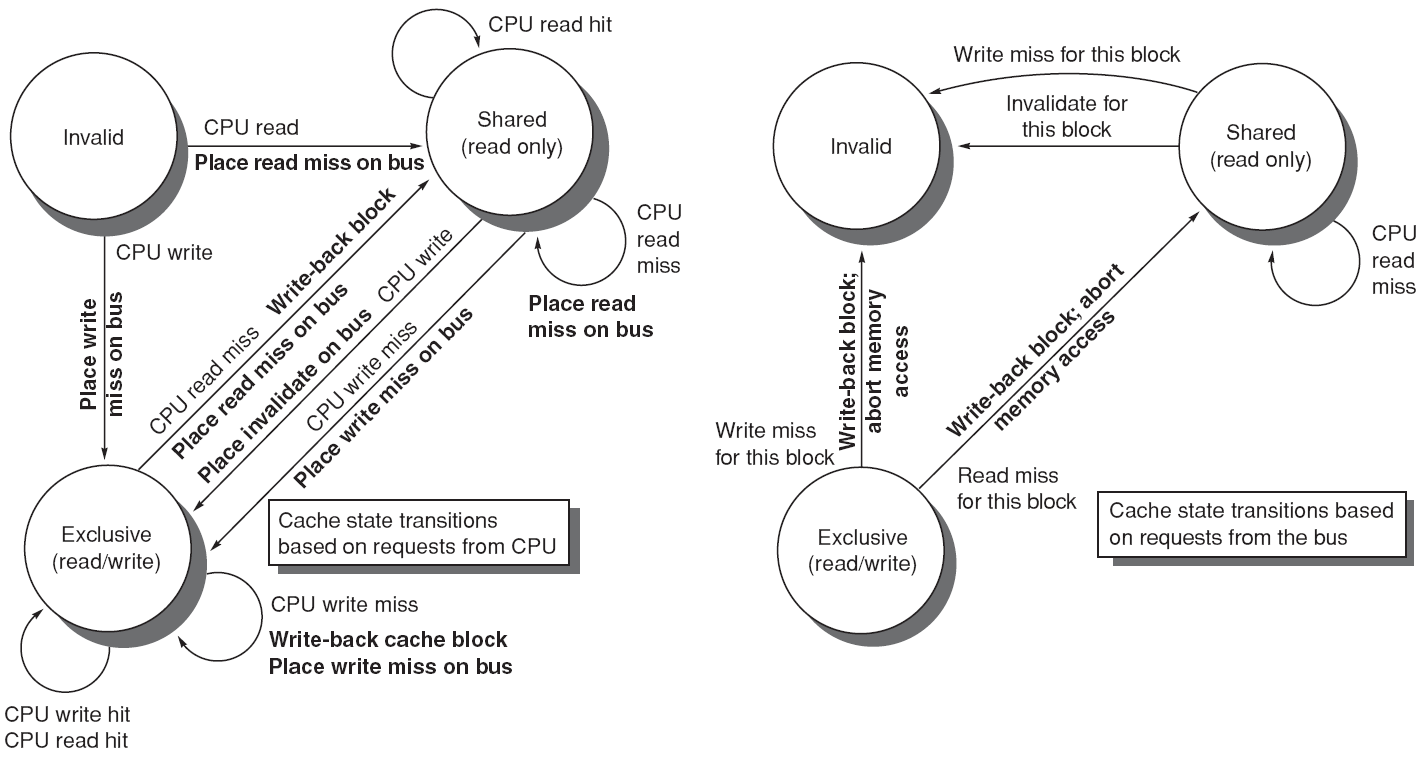
\includegraphics[scale=0.5]{img/snooping.png}
        \caption{Snooping states.}
        \label{img:snooping}
    \end{figure}
\end{theorem}

\item \begin{theorem}{()} \quad\quad \begin{itemize}
        \item NUMA is intrinsic in Von Neumann's computer model.
        \item Physical caches do NOT flush at \textbf{context switching}.
        \item Hyper-threading is \textbf{superscalar} and it can speedup \textbf{context switching}.
        \item Out-of-order execution in \textbf{cache} level do NOT fail.
        \item Data fault: Access invalid data memory, which is signaled by \textbf{MMU}.
        \item GPGPU usually runs \textbf{SPMT} (Single Program Multiple Thread), and GPU runs SIMT.
        \item L1 data cache is usually seperated from L1 instruction cache to \textbf{increase bandwidth}.
        \item Data cache is usually deployed at \textbf{MEM} stage.
        \item Increasing number of \textbf{used sticky bits} do NOT improve accuracy.
        \item \textbf{Memory hazard }do NOT cause stall, e.g. \code{sw} after \code{lw}.
        \item Branch target buffer is used by \textbf{CPU}.
    \end{itemize}
\end{theorem}
